\documentclass[04_projectProcess.tex]{subfiles}
\begin{document}
    \subsection{Related Work}
        \begin{flushleft}
            Many products are related to this project because many products deal with lightning.
            Light is very important for humans.\\~\\
            It gives us a hint about the time, when we should go sleeping and when we should get 
            up. The biological rhythm helps us in our daily life. In addition to this, the color 
            of the light helps us to create a form of atmosphere in certain situations.\\
            
            One product that deals with light are a common work light. It is less expensive and 
            people can only say if they want the light on or off. There are no other 
            functionalities. Still, nearly anyone has such a lamp in his/her office. \\

            However, the number of functions of these lamps is limited. That's why companies 
            gave them additional functions like changing the color. Usually, this can be done 
            by a smartphone app. There, people can define the color of the room. Furthermore, 
            they can define a time when the lamp has to switch on or off. A product that can 
            change its color is the Philip Hue lamps. In this ecosystem, people can do all this 
            in an app.  \\ 

            Still, there is no lamp you can interact with as you do with this one. Here, it 
            allows you to interactand to engage with the lamp again. Furthermore, there is no 
            need for using an app on the smartphone. So, there is less distraction, and anyone 
            can use it. Older people or very young people have problems using a smartphone. 
            People have to find the right app, have to understand how it works and also have to 
            define the new colors they want to use. That's why the idea of having a lamp you can 
            interact with and to change the color and the brightness, perhaps is a good one. \\~\\

            We have been inspired by a flexiable wood notebook that has been found in summer. 
            There, the cover of the the book was out of wood. If you opened it the back of the
            book lighted up (see Figure \ref{fig:inspirationLightUp}) and by closing it the 
            light switched off (see Figure \ref{fig:inspirationLightOff}). This was the 
            inspiration of the whole idea. We know we wanted to do something with flexiable 
            wood and with light. Because of our background, we add some interaction functionalities,
            so we came up with this idea.

            \begin{figure}[H]
                \centering
                \begin{subfigure}{.45\textwidth}
                    \centering
                    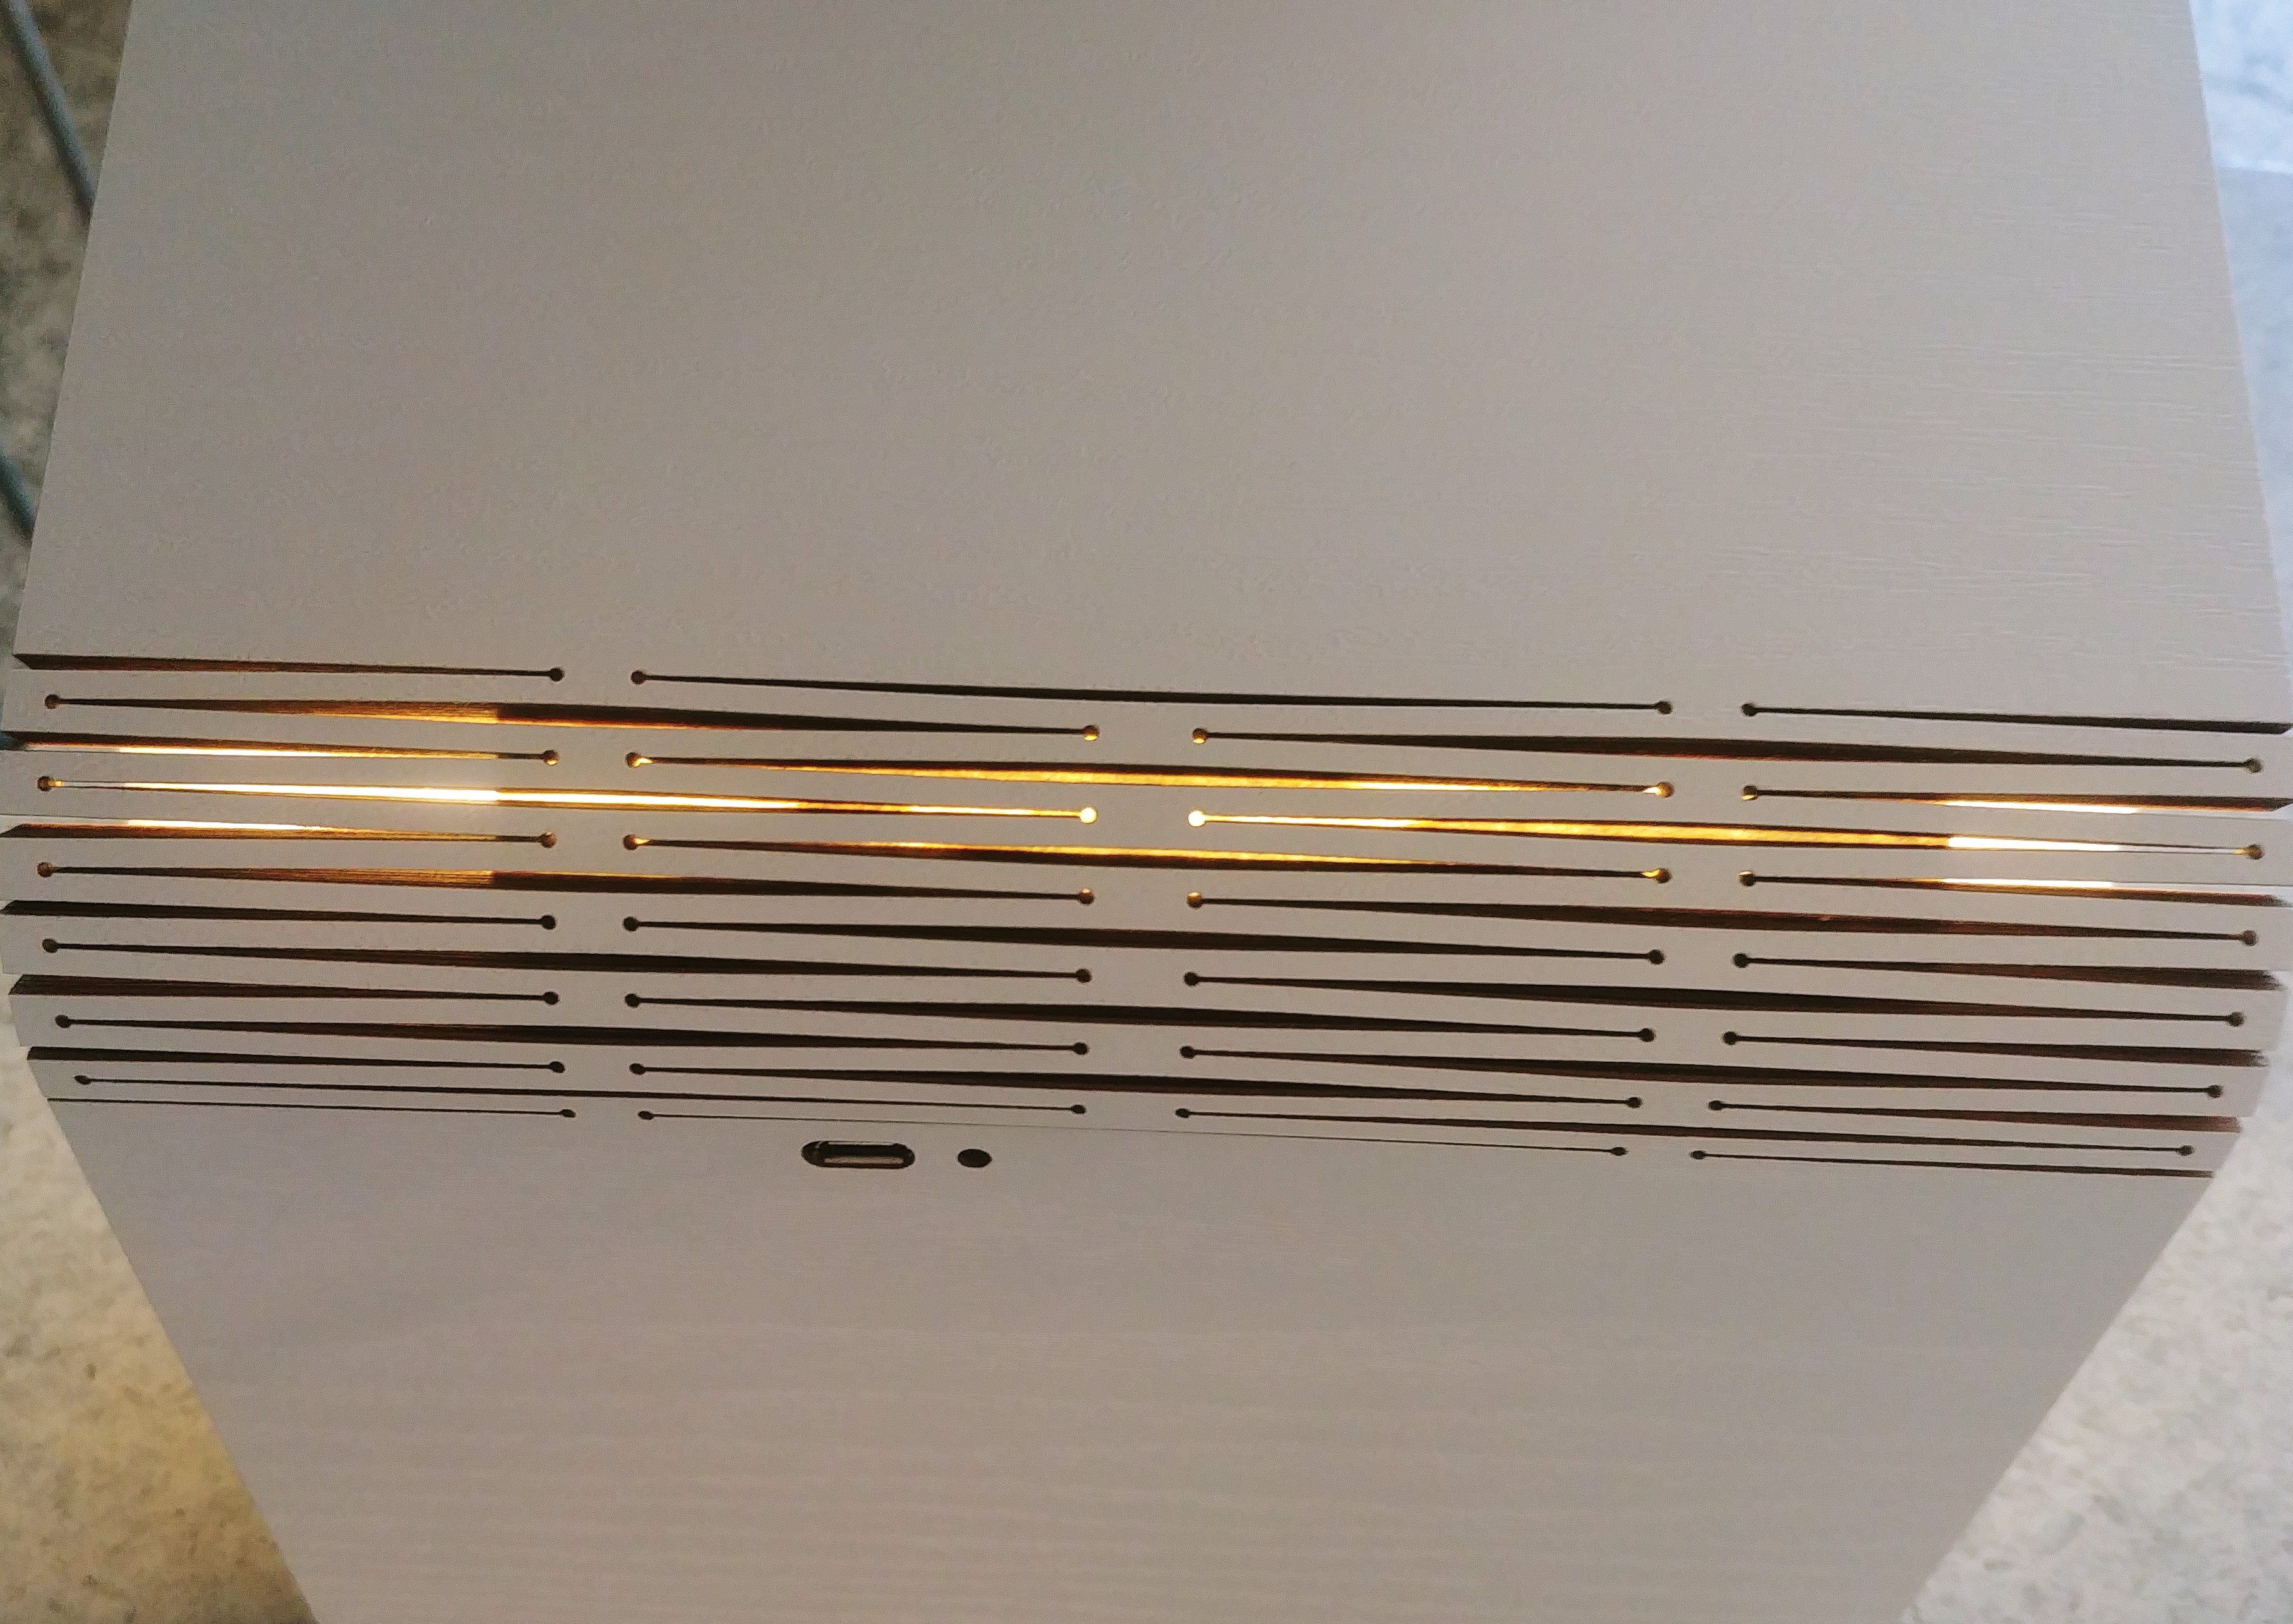
\includegraphics[width=0.8\linewidth]{images/projectideas/inspiration_on.jpg}
                    \caption{Shows the notebook open and light up.}
                    \label{fig:inspirationLightUp}
                \vspace{6mm}
                \end{subfigure}
                \begin{subfigure}{.45\textwidth}
                    \centering
                    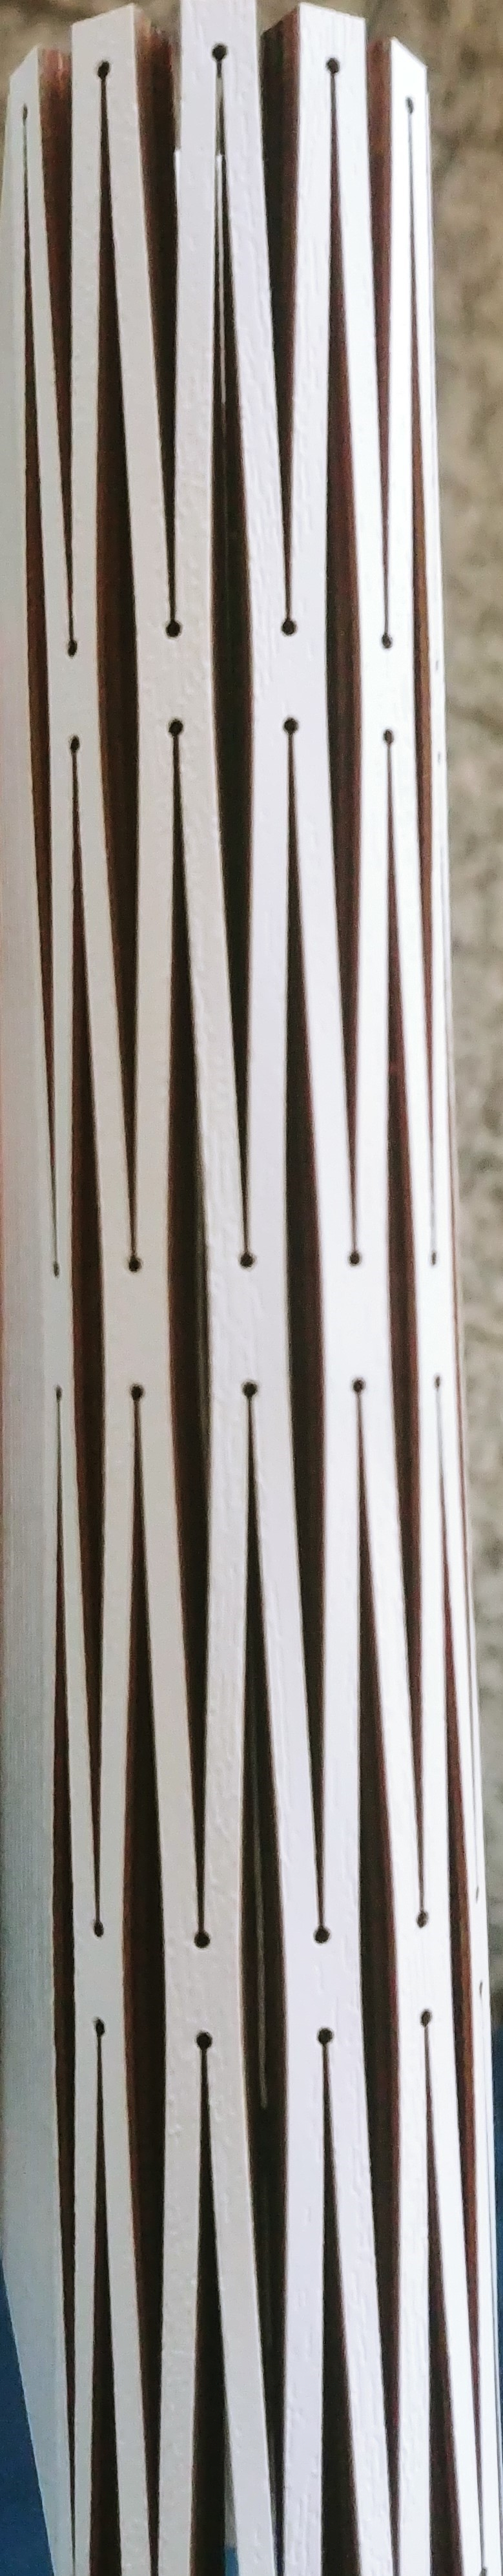
\includegraphics[scale=0.03, angle=90]{images/projectideas/inspiration_off.jpg}
                    \caption{Shows the notebook close and light off.}
                    \label{fig:inspirationLightOff}
                    \vspace{6mm}
                \end{subfigure}
                \caption{Shows the inspiration we had.}
                \label{fig:inspiration}
            \end{figure}
        \end{flushleft}
\end{document}
